\section{Analytical results}

\begin{wrapfigure}{R}{0.4\linewidth}
    \vspace*{-1cm}
    \centering
    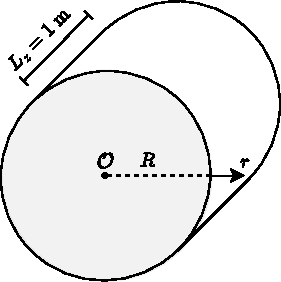
\includegraphics[width=\linewidth]{figures/cylindre.pdf}
    \caption{Cylinder of radius \(R\) inside heat source}
    \label{fig:gros_cylindre_uwu}
    \vspace*{1cm}
\end{wrapfigure}
The volume $\Omega$ is a cylinder of radius $R$ and length $L$ along the $\hat{z}$ axis, as shown in \autoref{fig:gros_cylindre_uwu}. It is made of inhomogeneous matter with thermal conductivity $\kappa(\vec{x})$ and has a heat source $S(\vec{x})$. It is placed in a thermal bath at $T_R$. We consider the temperature profile $T(\vec{x})$ at the stationary state.

\subsection{Differential Equation}
\underline{Question (a)}
We are searching for the differential equation of $T(\vec{x})$. We first give the continuity equation for the transfer of heat:
\begin{equation}
    \vec{\nabla} \cdot \vec{\jmath}_Q(\vec{x}) = S(\vec{x})
    \label{eq:continuity}
\end{equation}
where $\vec{\jmath}_Q$ is the heat flux. It is given by the diffusion:
\begin{equation}
    \vec{\jmath}_Q(\vec{x}) = -\kappa (\vec{x}) \vec{\nabla}T(\vec{x})
    \label{eq:heat_flux}
\end{equation}
Plugging \autoref{eq:heat_flux} into \autoref{eq:continuity} gives the equation:
\begin{equation}
    \vec{\nabla} \cdot (-\kappa(\vec{x})\vec{\nabla}T(\vec{x})) = S(\vec{x})
    \label{eq:true_equa_diff}
\end{equation}
which can be developped to give:
\begin{equation}
    \vec{\nabla}^2(T(\vec{x})) + \frac{1}{\kappa(\vec{x})} \vec{\nabla}(\kappa(\vec{x})) \cdot \vec{\nabla}(T(\vec{x})) + \frac{S(\vec{x})}{\kappa(\vec{x})} = 0
    \label{eq:equa_diff_T}
\end{equation}
the differential equation according to positions for $T(\vec{x})$.

\subsection{Weak formulation}
\underline{Question (b)}
We work towards the weak formulation of \autoref{eq:true_equa_diff} using $\eta \in \mathrm{C}^1(\Omega), \, \eta(\vec{x}) = 0 \,\forall \vec{x} \in \partial\Omega$:
\begin{equation}
    \begin{aligned}
        & -\vec{\nabla} \cdot (\kappa(\vec{x})\vec{\nabla}T(\vec{x})) = S(\vec{x}) \\
        & \Rightarrow -\eta(\vec{x}) \vec{\nabla} \cdot (\kappa(\vec{x})\vec{\nabla}T(\vec{x})) = \eta(\vec{x}) S(\vec{x})
    \end{aligned}
    \label{eq:weak_formulation_local}
\end{equation}

We then use:
\begin{equation}
    -\eta(\vec{x})\vec{\nabla}\cdot(\kappa(\vec{x})\vec{\nabla}T(\vec{x})) = \vec{\nabla}(\eta(\vec{x}))\cdot(\kappa(\vec{x})\vec{\nabla}T(\vec{x})) - \vec{\nabla}\cdot(\eta(\vec{x})\kappa(\vec{x})\vec{\nabla}T(\vec{x}))
\end{equation}
to have \autoref{eq:weak_formulation_local} as:
\begin{equation}
    \vec{\nabla}(\eta(\vec{x}))\cdot(\kappa(\vec{x})\vec{\nabla}T(\vec{x})) - \vec{\nabla}\cdot(\eta(\vec{x})\kappa(\vec{x})\vec{\nabla}T(\vec{x})) = \eta(\vec{x})S(\vec{x})
\end{equation}

This expression is then integrated over the whole cylinder $\Omega$ to have the weak formulation of the equation for $T$ and using the divergence theorem we find:
\begin{equation}
    \begin{aligned}
        & \iiint_\Omega \vec{\nabla}(\eta(\vec{x}))\cdot(\kappa(\vec{x})\vec{\nabla}T(\vec{x})) \mathrm{d}\Omega - \iiint_\Omega \vec{\nabla}\cdot(\eta(\vec{x})\kappa(\vec{x})\vec{\nabla}T(\vec{x})) \mathrm{d}\Omega = \iiint_\Omega \eta(\vec{x})S(\vec{x}) \mathrm{d}\Omega \\
        & \Rightarrow \iiint_\Omega \vec{\nabla}(\eta(\vec{x}))\cdot(\kappa(\vec{x})\vec{\nabla}T(\vec{x})) \mathrm{d}\Omega - \varoiint_{\partial\Omega} \eta(\vec{x})\kappa(\vec{x})\vec{\nabla}T(\vec{x}) \cdot \mathrm{d}\vec{\sigma} = \iiint_\Omega \eta(\vec{x})S(\vec{x}) \mathrm{d}\Omega
    \end{aligned}
    \label{eq:integrals}
\end{equation}
with the $\mathrm{d}\vec{\sigma}$ being the surface element vector. We have that $\eta(\vec{x}) = 0, \, \forall \vec{x} \in \partial\Omega$ so the closed integral in \autoref{eq:integrals} is 0 and:

\begin{equation}
    \iiint_\Omega \vec{\nabla}(\eta(\vec{x}))\cdot(\kappa(\vec{x})\vec{\nabla}T(\vec{x})) \mathrm{d}\Omega = \iiint_\Omega \eta(\vec{x})S(\vec{x}) \mathrm{d}\Omega
    \label{eq:weak_formulation}
\end{equation}

is the final weak formulation.

\subsection{Cylindrical coordinates}
\underline{Question (c)}
We now introduce cylindrical symmetry in the problem to have that:
\begin{equation}
    \frac{\partial}{\partial \varphi} = 0 \, ,\quad \frac{\partial}{\partial z} = 0
\end{equation}
and
\begin{equation}
    T(\vec{x}) = T(r) \, , \quad S(\vec{x}) = S(r) \, , \quad \kappa(\vec{x}) = \kappa(r) \, , \quad \eta(\vec{x}) = \eta(r)
\end{equation}
from the derivatives along $\varphi$ and $z$ being 0. This also allows to simplify the gradient in cylindrical coordinates:
\begin{equation}
    \vec{\nabla} = \left(\frac{\partial}{\partial r}, \frac{1}{r}\frac{\partial}{\partial \varphi}, \frac{\partial}{\partial z}\right) = \left(\frac{\partial}{\partial r}, 0, 0\right)
\end{equation}
Thus the weak formulation of \autoref{eq:weak_formulation} becomes:
\begin{equation}
    \iiint_\Omega \frac{\partial \eta (r)}{\partial r} \kappa(r) \frac{\partial T(r)}{\partial r} \mathrm{d}\Omega = \iiint_\Omega \eta(r)S(r) \mathrm{d}\Omega
\end{equation}
Still using cylindrical symmetry we also have $\frac{\partial}{\partial r} = \frac{\mathrm{d}}{\mathrm{d}r}$ as well as $\iiint_\Omega \mathrm{d}\Omega = 2\pi L \int_0^R r \mathrm{d}r$. This gives by simplifying the $2\pi L$ term on both sides:

\begin{equation}
    \int_0^R \frac{\mathrm{d} \eta (r)}{\mathrm{d} r} \kappa(r) \frac{\mathrm{d} T(r)}{\mathrm{d} r} r \mathrm{d}r = \int_0^R \eta(r)S(r) r \mathrm{d}r
    \label{eq:formulation_cylindrical}
\end{equation}

the weak formulation in cylindrical coordinates assuming cylindrical symmetry.

\subsection{Finite elements}
\underline{Question (d)}
We now want to apply $N$ finite linear elements $\{\Lambda_i(r)\}_{i=1,\ldots,N}$ defined for any mesh $\{r_i\}_{i=1,\ldots,N}$ representing the entire radius of the cylinder. For any $i \in \{2,\ldots,N-1\}$ the function $\Lambda_i(r)$ is defined on $[r_{i-1}, r_{i+1}]$ as:
\begin{equation}
    \Lambda_i(r) = \begin{cases}
        \frac{1}{r_i - r_{i-1}}(r - r_{i-1}) \quad , r \in [r_{i-1}, r_i] \\
        \frac{1}{r_{i+1} - r_i}(r_{i+1} - r) \quad , r \in \,\, ]r_i, r_{i+1}]
    \end{cases}
\end{equation}
with similar cases for $i=0$ and $i=N$ with only half of the domain.

We take $\{\eta_i\}_{i=1,\ldots,N}$ and $\{T_j\}_{j=1,\ldots,N}$ such that:
\begin{equation}
    \begin{aligned}
        & \eta(r) \approx \sum_{i=1}^N \eta_i \Lambda_i(r) \\
        & T(r) \approx \sum_{j=1}^N T_j \Lambda_j(r)
    \end{aligned}
\end{equation}

We have a freedom of choice for $\eta$ so any $\{\eta_i\}$ is viable as long as $\eta_N = \eta(r_N) = \eta(R) = 0$.
\autoref{eq:formulation_cylindrical} now becomes:
\begin{equation}
    \sum_{i=1}^{N} \sum_{j=1}^{N} \eta_i T_j \underbrace{\int_0^R \frac{\mathrm{d} \Lambda_i(r)}{\mathrm{d} r} \frac{\mathrm{d} \Lambda_j(r)}{\mathrm{d} r} \kappa(r)  r \mathrm{d}r}_{A_{ij}}  = \sum_{i=1}^{N} \eta_i \underbrace{\int_0^R \Lambda_i(r) S(r) r \mathrm{d}r}_{b_i}
    \label{eq:matrix_defs}
\end{equation}
with $\mathbf{A}$ an $N\times N$ matrix and $\vec{b}$ an $N$-dimensional vector. We thus have:
\begin{equation}
    \begin{aligned}
        & \sum_{i=1}^{N} \sum_{j=1}^{N} \eta_i T_j A_{ij}  = \sum_{i=1}^{N} \eta_i b_i \quad , \forall \{\eta_i\}, \eta_N = 0 \\
        & \Rightarrow \sum_{j=1}^{N} T_j A_{ij} = b_i \\
        & \Rightarrow \vec{T} \mathbf{A} = \vec{b}
    \end{aligned}
    \label{eq:system_of_equations}
\end{equation}
with $\vec{T}$ the vector corresponding to the set $\{T_j\}_{j=1,\ldots,N}$.

From \autoref{eq:matrix_defs} we can calculate \(\mathbf{A}\) using a loop over the intervals \(h_k = r_{k+1} - r_k\), \(k = 1, \dots, n\). Then we have
\begin{equation}
    A_{ij}
    = \int_0^R \frac{\dd \Lambda_i(r)}{\dd r} \frac{\dd \Lambda_j(r)}{\dd r} \kappa(r) r \dd r
    = \sum_{k=1}^n \underbrace{\int_{r_k}^{r_{k+1}} \frac{\dd \Lambda_i(r)}{\dd r} \frac{\dd \Lambda_j(r)}{\dd r} \kappa(r) r \dd r}_{C_{ij}^{(k)}}
\end{equation}
Because \(\frac{\dd \Lambda_i(r)}{\dd r} = 0\) outside of \([r_{i-1}, r_{i+1}]\), \(C^{(k)}_{ij}\) is nonzero if \((i,j) \in \{(k,k), (k+1,k), (k,k+1), (k+1,k+1)\}\). We then get
\begin{align*}
    C^{(k)}_{kk} &= \int_{r_{k}}^{r_{k+1}} \frac{\dd \Lambda_{k}(r)}{\dd r} \frac{\dd \Lambda_{k}(r)}{\dd r} \kappa(r) r \dd r = \int_{r_{k}}^{r_{k+1}} \frac{-1}{h_k} \frac{-1}{h_k} \kappa(r) r \dd r \\
    C^{(k)}_{(k+1)k} &= \int_{r_{k}}^{r_{k+1}} \frac{\dd \Lambda_{k+1}(r)}{\dd r} \frac{\dd \Lambda_{k}(r)}{\dd r} \kappa(r) r \dd r = \int_{r_{k}}^{r_{k+1}} \frac{1}{h_k} \frac{-1}{h_k} \kappa(r) r \dd r \\
    C^{(k)}_{k(k+1)} &= \int_{r_{k}}^{r_{k+1}} \frac{\dd \Lambda_{k}(r)}{\dd r} \frac{\dd \Lambda_{k+1}(r)}{\dd r} \kappa(r) r \dd r = \int_{r_{k}}^{r_{k+1}} \frac{-1}{h_k} \frac{1}{h_k} \kappa(r) r \dd r \\
    C^{(k)}_{(k+1)(k+1)} &= \int_{r_{k}}^{r_{k+1}} \frac{\dd \Lambda_{k+1}(r)}{\dd r} \frac{\dd \Lambda_{k+1}(r)}{\dd r} \kappa(r) r \dd r = \int_{r_{k}}^{r_{k+1}} \frac{1}{h_k} \frac{1}{h_k} \kappa(r) r \dd r \\
    C^{(k)}_{ij} &= 0 \textrm{ if } (i,j) \notin \{(k,k), (k+1,k), (k,k+1), (k+1,k+1)\}
\end{align*}
We can see from this that \(\mathbf{A} = \sum_{k=1}^{n} \mathbf{C}^{(k)}\) is tridiagonal. We follow the same process for \(\vec{b}\):
\begin{equation}
    b_i = \int_0^R \Lambda_i(r) S(r) r \dd r = \sum_{k=1}^{n} \underbrace{\int_{x_k}^{x_{k+1}} \Lambda_i(r) S(r) r \dd r}_{d^{(k)}_i}
\end{equation}
Because \(\Lambda_i(r) = 0\) outside of \([r_{i-1}, r_{i+1}]\), \(d^{(k)}_i\) is nonzero if \(i \in \{k, k+1\}\)
\begin{align*}
    d^{(k)}_k = \int_{x_k}^{x_{k+1}} \Lambda_k(r) S(r) r \dd r \\
    d^{(k)}_{k+1} = \int_{x_k}^{x_{k+1}} \Lambda_{k+1}(r) S(r) r \dd r
\end{align*}
And finally \(\vec{b} = \sum_{k=1}^{n} \overrightarrow{d^{(k)}}\). In order to apply the border conditions \(T(R) = T_R\), we need to change the last row of our system of equations shown in \autoref{eq:system_of_equations} such that \(T_n = T_R\). This means that we need to impose
\begin{equation}
    A_{nn} = 1, \quad A_{n(n-1)} = 0, \quad b_n = T_R
\end{equation}

\subsection{Analytical solution for homogeneous case}
\label{sec:solution_anal}
\underline{Question (e)}
From \autoref{eq:true_equa_diff} and cylindrical symmetry we have:
\begin{equation}
    \begin{aligned}
        & -\vec{\nabla} \cdot (\kappa(r)\vec{\nabla}T(r)) = S(r) \\
        & \Rightarrow -\frac{1}{r}\frac{\mathrm{d}}{\mathrm{d} r}\left(r \kappa(r) \frac{\mathrm{d}T}{\mathrm{d}r}(r)\right) = S(r)
    \end{aligned}
\end{equation}
which is the second order differential equation we want the analytical solution for. We have the conditions $S(r) = S_0$ and $\kappa(r) = \kappa_0$ which implies:
\begin{equation}
    \begin{aligned}
        & -\frac{\kappa_0}{r}\frac{\mathrm{d}}{\mathrm{d}r}\left(r\frac{\mathrm{d}T}{\mathrm{d}r}(r)\right) = S_0 \\
        & \Rightarrow \frac{\mathrm{d}T}{\mathrm{d}r}(r) + r\frac{\mathrm{d}^2T}{\mathrm{d}r^2}(r) = -\frac{S_0 r}{\kappa_0}
    \end{aligned}
\end{equation}
setting $\frac{\mathrm{d}T}{\mathrm{d}r}(r) = \Pi(r)$ to solve a first order equation first we have:
\begin{equation}
    \Pi + r\frac{\mathrm{d}\Pi}{\mathrm{d}r} = -\frac{S_0 r}{\kappa_0}
    \label{eq:first_order_ode}
\end{equation}

The homogeneous differential equation $\Pi + r\frac{\mathrm{d}\Pi}{\mathrm{d}r} = 0$ has solution:
\begin{equation}
    \Pi_H(r) = \frac{c_1}{r} \quad, \forall c_1\in\mathbb{R}
\end{equation}
We also find the particular solution from intuition:
\begin{equation}
    \begin{aligned}
        \Pi_p(r) = \frac{-S_0}{2\kappa_0}r
        \Rightarrow \Pi_p + r\frac{\mathrm{d}\Pi_p}{\mathrm{d}r} = \frac{-S_0}{2\kappa_0}r + r\frac{-S_0}{2\kappa_0} = -\frac{rS_0}{\kappa_0}
    \end{aligned}
\end{equation}
Thus the general solution of \autoref{eq:first_order_ode} is:
\begin{equation}
    \frac{\mathrm{d}T}{\mathrm{d}r}(r) = \Pi(r) = \frac{-S_0}{2\kappa_0}r + \frac{c_1}{r} \quad, \forall c_1\in\mathbb{R}
    \label{eq:sol_first_order_ode}
\end{equation}
which by integration gives:
\begin{equation}
    T(r) = -\frac{S_0}{4\kappa_0}r^2 + c_1\ln(r) + c_2 \quad, \forall c_1, c_2\in\mathbb{R}
\end{equation}
To find the specific solution for our problem we first know that the temperature is finite inside the cylinder and in particular at $r=0$. When $r\to0$ then $\ln(r)\to-\infty$ so this term must be deleted for the solution to be physical and then $c_1=0$.

We also have that the cylinder is in a thermal bath at $T_R$ so $T(R) = T_R$ and then:
\begin{equation}
    \begin{aligned}
        & T_R = T(R) = -\frac{S_0}{4\kappa_0}R^2 + c_2 \\
        & \Rightarrow c_2 = T_R + \frac{S_0}{4\kappa_0}R^2
    \end{aligned}
\end{equation}
and as a result our final solution for the temperature is:
\begin{equation}
    T(r) = \frac{S_0}{4\kappa_0}(R^2 - r^2) + T_R
    \label{eq:analytical_solution_T}
\end{equation}

We can also find from \autoref{eq:sol_first_order_ode} the solution for the heat flux to be:
\begin{equation}
    j_Q(r) = -\kappa(r)\frac{\mathrm{d}T}{\mathrm{d}r}(r) = \frac{S_0}{2}r
\end{equation}
